\chapter{The Pursuit of Majorana Fermions \label{chap:Majorana}}

The  Majorana Fermions, so called in the name of the Italian physicist Ettore Majorana, were first defined in the attempt to find a real solution of the Dirac equation. The real field that solves this equation describes a fermion which is its own antiparticle. Hence it has no electric charge  nor mass.  Till these days, no fundamental particle with these characteristics has been observed. However, in the last decade, there has been a huge speculation about the possibility of finding Majorana Fermions as a quasi-particles of certain types of topological superconductors.

The topological materials are a novel type of material that experiences phase transitions without any symmetry breaking. As consequence, they cannot be characterized by the Landau theory. Instead, the phase transition is characterized with a topological order . Since topological characters are discrete parameters that describe non-local features of the material, the phases with this characterization present robust characteristics that are difficult to alter. An example of this is the quantum hall effect which robustness is famous and widely used in high precision devices. 

One of the most promising topological materials is the one dimensional majorana wire. This wire is inspired in a famous Kitaev's toy model representing a spinless p-wave superconducting wire. Under certain conditions, the majorana wires experience topological phase transition characterized by the emergence exotic zero-modes localized at edges of the wire. Kitaev associated these modes with majorana quasi-particles  appearing at the boundary of the topological superconducting wire. Moreover, he pointed out that the combined used of robustness from topological materials and Majorana's non-abelian statistics could lead to the creation of fault tolerant quantum gates. This fact opened the doors to the search of majorana fermions in condensed matter physics. 

In this chapter we will present a review of the main topics about majorana fermions. In the first section \ref{sec:KitaevChain}, we will describe the the Kitaev's chain and the emergence of majorana zero modes. Next, we will discuss about the real implementations of majorana chains and the experimental proposals that have been carried on . Finally, we will take a look to the results coupling QDs with majorana chains.


% ------------------------Section: Kitaev *------------------
\section{The Kitaev Chain \label{sec:KitaevChain}}
In this section we discuss the main aspects of Kitaev's toy model. This is a toy model in tight binding that represents a  finite $p$-wave superconducting wire with the following Hamiltonian

\begin{equation}
H = \sum_{i=1}^N \left[ -t(a_i^{\dagger} a_{i+1} + a_{i+1}^{\dagger}a_i) -\mu a_i^{\dagger} a_{i} +  \Delta a_{i}a_{i+1} + \Delta^* a_{i+1}^{\dagger}a_i^{\dagger} \right].  \label{eq:kitaevHam}
\end{equation}

Where $\mu$ is the chemical potential, so that $\mu a_i^{\dagger} a_{i}$ is the energy associated to each step in the chain. $t(a_i^{\dagger} a_{i+1} + a_{i+1}^{\dagger}a_i)$ represents the interaction between neighbouring sites which is determined by the hopping term $t$. The remaining terms describe the superconducting properties of the system as is is established by the BCS theory of superconductivity. $\Delta$ is a complex superconducting parameter with the form  $\Delta = e^{i\theta} \super$. The associated terms represent the Cooper pairs which can be created or annihilated at neighbouring sites of the system.

The form of hamiltonian \prettyref{eq:kitaevHam} favors the possibility of introducing new operators $\gammaA{j}$ and $\gammaB{j}$ such that

\begin{equation}
\gammaA{j} = e^{i\theta /2}a_j+ e^{-i\theta/2 } \ann_j \ \ , \ \ \gammaB{j} = -i(e^{i\theta /2}a_j - e^{-i\theta/2} \ann_j).
\label{eq:majoranaTrans}
\end{equation}
It is simple check that these operators are self-adjoint $(\gammaA{j}^\dagger = \gammaA{j}, \gammaA{j}^\dagger = \gammaB{j})$. This is a required constraint for the Majorana particles. In addition they satisfy the fermionic anti-commutation relations
\begin{equation}
\begin{aligned}
\{\gammaA{i}, \gammaA{j}\} = \{ & \gammaB{i} , \gammaB{j}\} = 2\delta_{ij}  ,\\ 
  \{\gammaA{i}, \gammaB{j} & \} =0.
\end{aligned} 
\label{majoranaRel}
\end{equation} 
This allows us to understand the operators $\gammaA{i} , \gammaB{i}$ as majorana fermions. If we also take the inverse of \prettyref{eq:majoranaTrans} we obtain that each  (Dirac) fermion in Hamiltonian \eqref{eq:kitaevHam} is composed by two majorana fermions such that 
$$a_j = \frac{e^{-i\theta/2}}{2}(\gammaA{j}+ i\gammaB{j})$$
We could even adventure to say that these majorana operators are actually dividing the Dirac fermions into real($\gammaA{}$) and imaginary $(\gammaB{})$ part ,the same way as complex numbers are a composite of two real numbers. 

The new Kitaev Hamiltonian in the Majorana representation looks like 

\begin{equation}
H = \frac{i}{2} \sum_{j=1}^N \left[ -\mu \gammaA{j}\gammaB{j}  + (t- \super) \gammaB{j}\gammaA{j+1} + (t+ \super) \gammaA{j}\gammaB{j+1} \right]+Const,\label{eq:HamMajorana}
\end{equation}

Depending on the values of parameters $\mu, t$ and $\super$ we can identify two regimes represented by the following situations:


%\begin{figure}[t]
%$$\includegraphics[scale=0.5]{KitaevtopPhases.jpg}
%\centering
%\label{top.phases kitaev}
%\caption{{\small \textit{Taken from \cite{bernevig2015topological}. Ilustration of the Kitaev chain for open boundary conditions in the Majorana representation. a)Represents the trivial case where the hopping and the superconducting term approaches to $0$. b) The non-trivial topological phase. The coupling is produced between Majoranas in different Dirac fermions }}}
%\end{figure}

\begin{figure}[hbt]
    \centering
    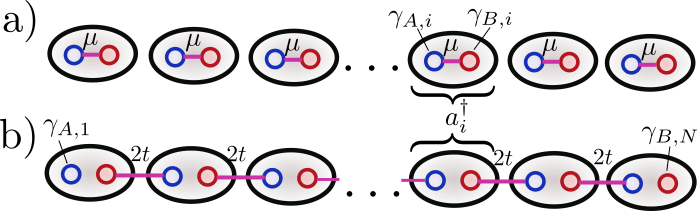
\includegraphics[scale=0.5]{IMAGES/Majorana/KitaevChain.png}
    \label{fig:top.phases kitaev}
    \caption{Illustration of the Kitaev chain for open boundary conditions in the Majorana representation. a)Represents the trivial case where the hopping and the superconducting term approaches to $0$. b) The non-trivial topological phase. The coupling is produced between Majoranas in different Dirac fermions \protect\Source{By the author} }
\end{figure}


\begin{enumerate}
\item{If $\super = t = 0, \mu <0$} Hamiltonian \eqref{eq:HamMajorana} becomes $\frac{-i\mu}{2} \sum_{j} \gammaA{j}\gammaB{j}$ which represents the coupling of the Majoranas in the same Dirac fermion. (See Figure \ref{fig:top.phases kitaev} (a))

\item{If $\super = t > 0, \mu =0$} the situation is much more interesting. The Hamiltonian \eqref{eq:HamMajorana} takes the form $H = 2ti\sum_{j} \gammaA{j}\gammaB{j+1}$. This implies that the coupling is performed between  Majoranas of different Dirac fermions leaving the edge Majorana operators ($\gammaA{1}$ and $\gammaB{N}$) uncoupled (See Figure \ref{fig:top.phases kitaev}b)). Note that these uncoupled majorana fermions can be at any state without any  repercussion in the energy of the system. This explains the emergence of a  ground state localized at edges of the chain. 
\end{enumerate}

These two situations are representatives of two different phases. The trivial phase occurs for $\frac{\mu}{2t}>1$ and the non-trivial phase appears when $\frac{\mu}{2t}<1$ (See figure \ref{fig:KitaevSpec}). The mean characteristic of the non-trivial phase is the creation of an stable zero-mode. This zero-mode is generated by the  uncoupled majorana fermions at the edges of the Kitaev chain.  \\



\begin{figure}[t]
    \centering
    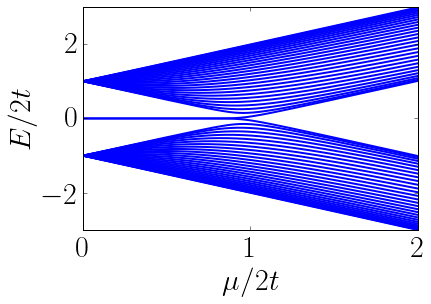
\includegraphics[scale=0.5]{IMAGES/Majorana/Spectrum.png}
    \label{fig:KitaevSpec}
    \caption{Spectrum of Hamiltonian \eqref{eq:HamMajorana} with $30$ sites and $t=\super$ s. Method: Numerical diagonalization. \protect \Source{By the author} }
\end{figure}



% ---------------Subsection: Topological phase transition-------------
\subsection{Topological phase transition}

The two regimes described previously  can be characterized with a topological parameter.  One of the methods for this is following the idea used by \citeauthor{alicea_new_2012}\cite{alicea_new_2012}. The first part is to suppose that we have an infinite chain $(N=\infty)$ in Hamiltonian \eqref{eq:HamMajorana}. The new system is translation invariant, hence we can make a transformation to the momentum space. Then we may rewrite Hamiltonian \eqref{eq:HamMajorana}  as

\begin{equation}
    H = 
    \sum_{k \in BZ} 
    \begin{pmatrix} 
      b_k'  & c_{k}'\\  
    \end{pmatrix}
    H_k 
    \begin{pmatrix} 
      b_{-k}'     \\ 
      c_{-k}' 
    \end{pmatrix}.
    \label{PBCHam2}
\end{equation}

with the Bloch Hamiltonian 

\begin{equation}
H_k = \begin{pmatrix} 
      0    &  \frac{-i \mu}{2} + it \cos k + \super  \sin k  \\ 
       \frac{i \mu}{2} - it \cos k + \super \sin k  &  0 
    \end{pmatrix}
    = (\super \sin k) \sigma_x + (\frac{\mu}{2}- t \cos k) \sigma_y.
\label{sigma}
\end{equation}




\noindent where $\sigma_x$ , $\sigma_y$ are the corresponding Pauli matrices. The Brilloin zone ($BZ$) is the periodic space  $[-\pi , \pi]$ which can be mapped to the unitary circle.   Equation \eqref{sigma} determines  the coordinates of the Bloch Hamiltonian in the base $\{\sigma_x, \sigma_y\}$. We can map these coordinates to the unitary circle by taking the norm of this vector giving
\begin{equation}
     \hat{H}_k= \frac{1}{\sqrt{\super^2 \sin^2 k + (\frac{\mu}{2}- t \cos k)^2}}
     \begin{pmatrix} 
      \super \sin k    \\ 
      \frac{\mu}{2}- t \cos k 
    \end{pmatrix}. 
\end{equation}

Note that $\super^2 \sin^2 k + (\frac{\mu}{2}- t \cos k)^2 \neq 0$ for all the values of $k$ as long as $\frac{\mu}{2t} \neq 1$ . When $\frac{\mu}{2t} = 1$ the $H_{k=0}=0$, so it cannot be normalized. \textbf{This is the same point were the phase transition occurs!}. At any other value of $\frac{\mu}{2t}$ it is possible to normalize $H_{k}$ for all values of $k\in BZ$. The result of mapping $\hat{H}_k$ for all $k$ is a path around the unitary circle. \\

This path can take two forms as we can observe in Figure \ref{fig:topological}. If $\frac{\mu}{2t} > 1$ the path reduced to a line in the upward part of the circle. In the non-trivial phase $\frac{\mu}{2t} < 1$ the path completes the round to the entire circle. Note that this method states a topological difference between the two phases. While the path described by the trivial phase can be contracted to a single dot, the path described by the non-trivial one is a circle that cannot be contracted. \\

Note that to determine whether path of a given phase is of type a) or type b) we only need to check if $\hat{H}_{k=0}$ and $\hat{H}_{k=\pi}$ are the same point or opposite points. This transforms into a simple equation 
\begin{equation}
    \hat{H}_{k=0,y}\hat{H}_{k=\pi,y}=\begin{cases}
1 & \mbox{trivial phase}\\
-1 & \mbox{non-trivial phase}
\end{cases}
\end{equation}
where $\hat{H}_{k=0,y}$ is the $y$-th component of $\hat{H}_{k}$. The term $\hat{H}_{k,y}$ is a particular case of the Pfaffian $\mathcal{P}(k)$, which widely used as topological order in  phases transition including  majorana modes . 


\begin{figure}[t]
    \centering
    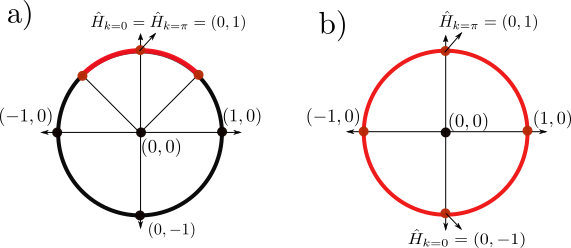
\includegraphics[scale=0.8]{IMAGES/Majorana/Topological.png}
    \label{fig:topological}
    \caption{ The following represents the path of $\hat{H}_k$ for the interval $[ -\pi, \pi ]$. a) Corresponds to the trivial phase. The resulting path can be homotopically deformed to a point. b) The non-trivial phase corresponds to a non-contractible loop around the unitary circle. \protect \Source{By the author}} 
\end{figure}

The mean idea behind this topological characterization relies in the adiabatic theorem.  In simple words, the adiabatic theorem says that a slow evolution of a gaped Hamiltonian will produce a smooth evolution of its ordered eigenstates. i.g The order of the eigenstates remains unchanged. \\

The keyword in the previous definition is "gaped". As we can observe in Figure \ref{fig:KitaevSpec} the phase transition occurs at $\frac{\mu}{2t}=1$. This is when the system transitions between a gapless and gaped Hamiltonians.  \\

The connection with topology comes from the fact that adiabatic evolutions can be understood as smooth deformations of the Hamiltonian. However since gapless Hamiltonians imply phase transitions, the theory defines the gapless points as holes (or forbidden points) in the phase space. Then characterizing the phase transitions in the Kitaev chain is mainly a topological problem where gaped Hamiltonians are holes in the topological space. In addition, the topological orders characterizing this transition will be Chern or Winding numbers. \\


Though this connection between physics and topology is quite interesting, I will stop here because it is taking us out of our real discussion which is majorana fermions.  You can find more information about this in ( \Jesus{add references}). 

% -----------------------Subsection: Non-abelian Statistics -------------
%\subsection{Non-abelian statistics}







% -----------------------Section: Modern and Experimental-------------
\section{Real implementations of Majorana Chains}
\Jesus{Here comes a summary of real models and implementations of majorana chains. I am still thinking how to write this section. For now, I leave some ideas}

Although the Kitaev chain its just a toy model, it does describes some interesting physics. 

The promise of finding the exotic majorana particles that could bring new insights to quantum computing motivated the implementation of real models that could emulate the physics of a Kitaev chain. 

Spin is a major problem. A material with spin-orbit coupling is  the solution to this situation. \ref{fig:sipin-orbit} 

\begin{equation}
    H =\int\mbox{d}x\psi^{\dagger}\left(\frac{\partial^{2}}{2m\partial x^{2}}-\mu -i\alpha\sigma_{y}\partial x+h\sigma_{x}\right)\psi+\Delta\psi_{\downarrow}\psi_{\uparrow}+\Delta^{*}\psi_{\downarrow}\psi_{\uparrow},
    \label{eq:MajoranaChainHam}
\end{equation}




\begin{figure}[t]
\centering
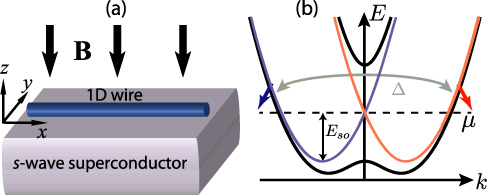
\includegraphics[scale=0.7]{IMAGES/Majorana/Mwire.png}

\caption{ \label{fig:spin-orbit} \protect\Source{\cite{alicea_new_2012}}}
\end{figure}

\begin{figure}[H]
\centering

     \subfloat[ \label{fig:exp1}]{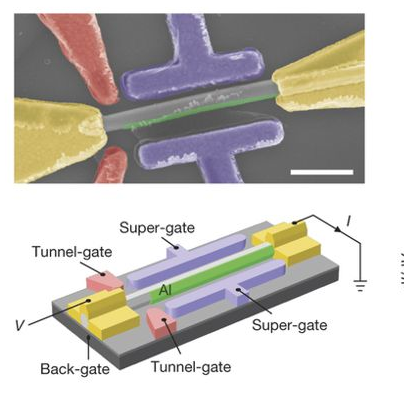
\includegraphics[scale=0.3]{IMAGES/Majorana/Exp.png}}  
     \subfloat[\label{fig:exp2}]{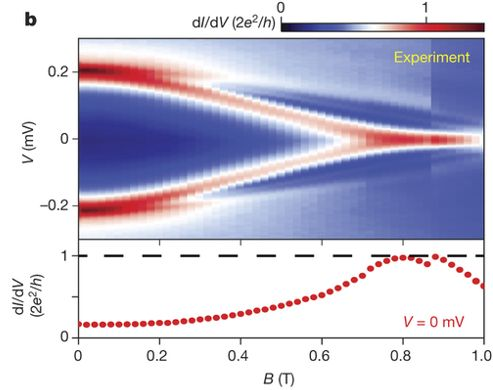
\includegraphics[scale=0.3]{IMAGES/Majorana/Exp2.png}}
\caption{ \label{ex}\protect\Source{\cite{zhang_quantized_2018}}}
\end{figure}


% -----------------------Leaking majorana modes in quantum dots-------------

\section{Coupling Majoranas to QDs}
\citeauthor{liu_detecting_2011} was one of the first in proposing the possibility of using QDs in the pursuit of Majorana fermions . When a QD is attached to a the end of a majorana chain in the topological phase,  the majorana mode at the end of the chain then leaks inside the QD \cite{vernek_subtle_2014}. This produces a zero-bias conductance peak of half a quanta $\frac{e^{2}}{2h}$ through the dot.

 We can reconstruct these results using the methods that we developed in \ref{chap: Methods}. To this lets first define our model hamiltonian:
\begin{equation}
    H=H_{QD-Lead}+H_{M-QD}+H_M.
\end{equation}
Where $H_{QD-Lead}$ is the Hamiltonian for the non-interacting Anderson model \eqref{eq:Anderson}, $H_M$ is the Hamiltonian of the majorana chain and $H_{M-QD}$ represents the coupling between the QD and the Majorana Fermion at the boundary.

Now, the real question is how to define the coupling between the QD and the majorana fermion. In fact, there are many ways to represent this interaction. One alternative is to replace in $H_{M}$ with the entire Kitaev chain hamiltonian \eqref{eq:kitaevHam} (or  even with the  majorana chain \eqref{eq:MajoranaChainHam}) and then pick $H_{M-QD}$ as a simple coupling between the QD and the first site of the chain \cite{vernek_subtle_2014}.  A simpler approach is  to define an effective coupling with the majorana operator at the edge of the majorana chain. Since the Kitaev chain is spin-less, we choose to couple the majorana to the spin-$\dw$ channel of the QD \footnote{An appropriate justification of this fact can be found in \cite{ruiz-tijerina_interaction_2015}} . Therefore, the majorana fermion should be the superposition of the creation and annihilation operators of a spin $\dw$ particle $f_\dw$:

$$\gamma_1 := \frac{1}{\sqrt{2}} \left( f^\dagger_{\dw} + f_{\dw}\ \right) , \gamma_2 := \frac{1}{\sqrt{2}} \left( f^\dagger_{\dw} - f_{\dw} \right).$$

This makes possible to define an effective coupling between the Majorana Mode and the dot by attaching $\gamma_1$ with the spin-$\dw$ channel in the QD

%H_{TS} & = & 2\epsilon_{m}\gamma_{1}\gamma_{2}\nonumber \\
\begin{eqnarray}
H_{M-QD} & = &  t_1 \left(d_{\downarrow}^{\dagger}\gamma_{1}+\gamma_{1}d_{\downarrow}\right) 
% \\
% & = &  \sum_{i}t_{i} \left(d_{i\downarrow}^{\dagger}f^\dagger_{\dw} + 
% f_{\downarrow}d_{i\dw} +d_{i\downarrow}^{\dagger}f_{\dw}+
% +f_{\downarrow}^{\dagger} d_{i\downarrow}\right).
\label{eq:MajoranaCoupling}
\end{eqnarray}




% \begin{equation}
%     \omega\Green{A,B} =\delta_{A^{\dagger},B}+\Green{\left[A,H\right],B}
% \end{equation}

Then the coupling with the chain is given by 

\begin{eqnarray*}
H_{M} & = & \epsilon_{m}f_{\downarrow}^{\dagger}f_{\downarrow}\\
H_{M-QD}&=&\frac{t_1}{\sqrt{2}}d_{1\downarrow}^{\dagger}f_{\downarrow}+\frac{t_1^{*}}{\sqrt{2}}f_{\downarrow}^{\dagger}d_{1\downarrow}+\frac{t_1}{\sqrt{2}}d_{1\downarrow}^{\dagger}f_{\downarrow}^{\dagger}+\frac{t_1^{*}}{\sqrt{2}}f_{\downarrow}d_{1\downarrow}
\end{eqnarray*}

Finally we obtain the following hamiltonian

\begin{equation}
H =\sum_{k,\sigma}\left(\epsilon_1+\frac{U_1}{2}\right)d_{1\sigma}^{\dagger}d_{1\sigma}+ \frac{U}{2}(d_{1\sigma}^{\dagger}d_{1\sigma}-1)^{2} + t_1 \left(d_{1\downarrow}^{\dagger}\gamma_{1}+\gamma_{1}d_{1\downarrow}\right) + Vd^\dagger_{1\sigma}c_{k\sigma}+V^* c^\dagger_{k\sigma}d_{1\sigma}+ \epsilon_{m}f_{\downarrow}^{\dagger}f_{\downarrow}.
\label{eq:QD-Mham}
\end{equation}


The fidelity of this effective model has been discussed by \citet{ruiz-tijerina_interaction_2015}
concluding that the majorana effective hamiltonian reproduces the
same results than the Kitaev chain model in the topological phase
(This statement is true even for more realistic models of the TS that
include Rashba spin-orbit interactions and a Zeeman field \citep{ruiz-tijerina_interaction_2015}
).\\


\subsection{Non-interacting ($U_1 = 0$) QD coupled to a Majorana chain}

In the non-interacting case we can use the ballistic transport equations from \ref{sec:transport}.The green functions are then determined by the following set of linear equations. 

\begin{figure}[t]
\centering
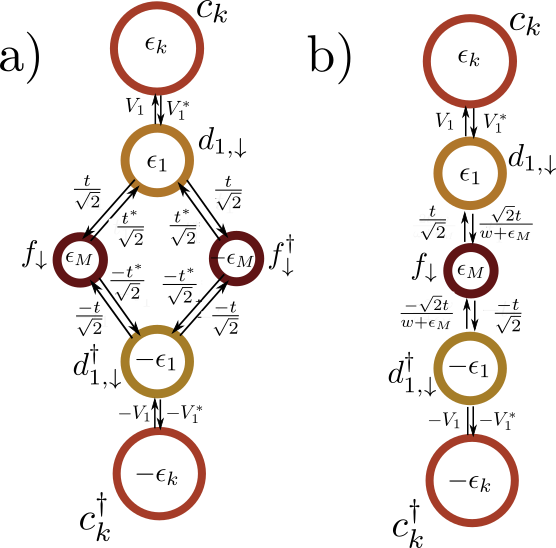
\includegraphics[scale=0.5]{IMAGES/Majorana/Grenn-Majorana.png}
\caption{ Graph $\GM$ representing the transport equations.  \label{fig:green-M-QD} \protect\Source{\cite{By the author}}}
\end{figure}


\begin{align}
    \left(\omega-\epsilon_{M}\right)\Green{f_{\downarrow},d_{1\downarrow}^{\dagger}}&=\left(\omega+\epsilon_{M}\right)\Green{f_{\downarrow}^{\dagger},d_{1\downarrow}^{\dagger}}=\frac{t^*_1}{\sqrt{2}}\left(\Green{d_{1\downarrow},d_{1\downarrow}^{\dagger}}-\Green{d_{1\downarrow}^{\dagger},d_{1\downarrow}^{\dagger}}\right)\\
    \left(\omega-\epsilon_{1}\right)\Green{d_{1\downarrow},d_{1\downarrow}^{\dagger}}&=1+\frac{t_1}{\sqrt{2}}t_{1}\Green{f_{\downarrow},d_{1\downarrow}^{\dagger}}+\frac{t_1}{\sqrt{2}}t_{1}\Green{f_{\downarrow}^{\dagger},d_{1\downarrow}^{\dagger}}+V_{1}\sum_{\mathbf{k}}\Green{c_{\mathbf{k\downarrow}},d_{1\downarrow}^{\dagger}}\\
    \left(\omega-\epsilon_{\mathbf{k}}\right)\Green{c_{\mathbf{k}},d_{1\downarrow}^{\dagger}}&=V_{1}^{*}\Green{d_{1\downarrow},d_{1\downarrow}^{\dagger}}\\
    \left(\omega+\epsilon_{1}\right)\Green{d_{1\downarrow}^{\dagger},d_{1\downarrow}^{\dagger}}&=-\frac{t_1}{\sqrt{2}}\Green{f_{\downarrow},d_{1\downarrow}^{\dagger}}-\frac{t_1}{\sqrt{2}}\Green{f_{\downarrow}^{\dagger},d_{1\downarrow}^{\dagger}}-V_{1}^{*}\sum_{\mathbf{k}}\Green{c_{\mathbf{k\downarrow}}^{\dagger},d_{1\downarrow}^{\dagger}}\\
    \left(\omega+\epsilon_{\mathbf{k}}\right)\Green{c^\dagger_{\mathbf{k}},d_{1\downarrow}^{\dagger}}&=-V_{1}^{*}\Green{d_{1\downarrow},d_{1\downarrow}^{\dagger}}
\end{align}

The graph representing these green functions is represented in \ref{fig:green-M-QD} a)  (Look \ref{sec:GraphMethod} for details). However using that $\left(\omega-\epsilon_{M}\right)\Green{f_{\downarrow},d_{1\downarrow}^{\dagger}}=\left(\omega+\epsilon_{M}\right)\Green{f_{\downarrow}^{\dagger},d_{1\downarrow}^{\dagger}}$ we can take
 $\Green{f_{\downarrow}^{\dagger},d_{1\downarrow}^{\dagger}}$ out of the equations getting the system in \ref{fig:green-M-QD} b) .  Following the graph method the green function for dot 1 is
\begin{equation}
    \Green{d_{1\downarrow},d_{1\downarrow}^{\dagger}}=\left[\omega-\epsilon_{1}-\sum_{\mathbf{k}}\frac{V_{1}V_{1}^{*}}{\omega-\epsilon_{1}}-\frac{\omega}{\omega+\epsilon_{M}}\frac{\left\Vert t\right\Vert ^{2}}{\left[\GreenG{f_{\downarrow},f_{\downarrow}^{\dagger}}{\GM-d_{1}}\right]^{-1}}\right]^{-1}.
\end{equation}
Hence we just need the green function of $\GreenG{f_{\downarrow},f_{\downarrow}^{\dagger}}{\GM-d_{1}}$ removing $d_1$ out of the graph. This case is much simpler since $f_\downarrow$ is just attached to $d^\dagger_1$ . Thus we get
\begin{equation}
    \GreenG{f_{\downarrow},f_{\downarrow}^{\dagger}}{\GM-d_{1}}=\left[\omega-\epsilon_{M}-\frac{\omega}{\omega+\epsilon_{M}}\frac{\left\Vert t\right\Vert ^{2}}{\omega+\epsilon_{1}-\sum_{\mathbf{k}}\frac{V_{1}V_{1}^{*}}{\omega-\epsilon_{\mathbf{k}}}}\right]^{-1}.
\end{equation}

Again, the only missing point in this equation is to replace $\sum \frac{V_1V^*_1}{\omega -\epsilon_k}= -i\Gamma_1$. Note that this computations are only for the spin-$\dw$ channel. The spin-$\up$ channel is even simpler since this channel is not coupled to the majorana mode. Hence it corresponds to the case of a single quantum dot coupled to a Lead.  The results for the DOS can be observed in \ref{fig:M1-Tot}. Each figure has an inset showing the model in the majorana representation. The small blue and red balls are majorana fermions just as the ones in figure \ref{fig:top.phases kitaev}. The majorana at the edge of the majorana chain is represented by the isolated red ball majorana connected to the QD (Figure \ref{fig:M1}). The other isolated blue ball in Figure \ref{fig:M1-em} represents the majorana at the other edge which is connected to the sphere by the parameter $\epsilon$. 

\begin{itemize}
    \item[\ref{fig:M1}] 
    \item[\ref{fig:M1-e1}]
    \item[\ref{fig:M1-em}]
\end{itemize}



\begin{figure}[t]
     \centering
    \subfloat[  \label{fig:M1}]{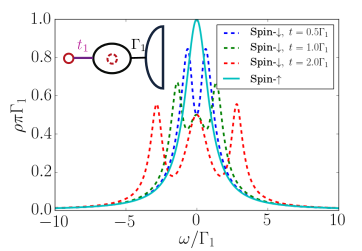
\includegraphics[scale=0.5]{IMAGES/Majorana/M1.png}}
     \subfloat[ \label{fig:M1-e1}]{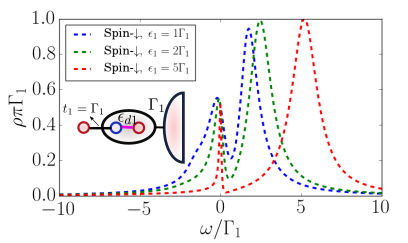
\includegraphics[scale=0.51]{IMAGES/Majorana/M1-e1.png}} 
    \subfloat[\label{fig:M1-em}]{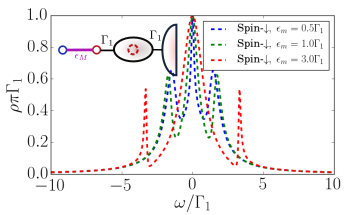
\includegraphics[scale=0.55]{IMAGES/Majorana/M1-eM.png}}
    
     \caption{\label{fig:M1-Tot} ..\Jesus{I don't like the variables of  the c) plot. So I might change them soon}.  \protect\Source{ By the Author  }}
\end{figure}




\subsection{NRG: Kondo-Majorana physics}
In the interacting 
\begin{figure}[t]
\centering
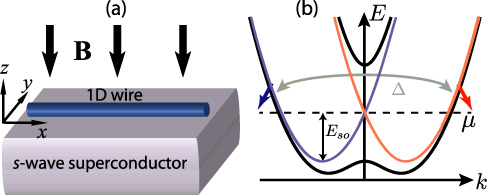
\includegraphics[scale=0.7]{IMAGES/Majorana/Mwire.png}

\caption{ \label{fig:NRG-1M} \protect\Source{\cite{By the author.}}}
\end{figure}


 \citeauthor{ruiz-tijerina_interaction_2015}  proved that this effective coupling  is able to reproduce efficiently the results obtained when the Kitaev chain in the topological phase is attached to a single QD. 

% \begin{eqnarray*}
% H_{TS} & = & 2\epsilon_{m}f_{\downarrow}^{\dagger}f_{\downarrow}-\epsilon_{m}\\
% H_{int} & = & \sum_{i}\tilde{t_{i-}}d_{i\downarrow}^{\dagger}f_{\downarrow}+\tilde{t_{i-}}^{*}f_{\downarrow}^{\dagger}d_{i\downarrow}+\tilde{t_{i+}}d_{i\downarrow}^{\dagger}f_{\downarrow}^{\dagger}+\tilde{t_{i+}}^{*}f_{\downarrow}d_{i\downarrow}
% \end{eqnarray*}

% with $\tilde{t}_{i\pm}=\frac{1}{\sqrt{2}}\left(\left|t_{i1}\right|-i\left|t_{i1}\right|e^{i\phi_{i}}\right).$



% so that 

% \[
% \gamma_{1}=\frac{1}{\sqrt{2}}\left(f_{\downarrow}^{\dagger}+f_{\downarrow}\right)\ ,\gamma_{2}=\frac{1}{i\sqrt{2}}\left(f_{\downarrow}^{\dagger}-f_{\downarrow}\right).
% \]


% \begin{eqnarray}
% H_{TS} & = & 2\epsilon_{m}\gamma_{1}\gamma_{2}\nonumber \\
% H_{int} & = & \sum_{i}t_{i1}\left(d_{i\downarrow}^{\dagger}\gamma_{1}+\gamma_{1}d_{i\downarrow}\right)+it_{i2}\left(d_{i\downarrow}^{\dagger}\gamma_{2}+\gamma_{2}d_{i\downarrow}\right),\label{eq:Majorana-ham}
% \end{eqnarray}


% where $\gamma_{1,2}$are the two majorana operators and$t_{i1,2}$
% are the hopping terms between the majoranas and the QDs.




% A Majorana chain coupled to a QD can be studied using the methods described in chapter \ref{chap: Methods}






% % where $H_{d_{i}}$is the QD hamiltonian for dot $i$ \prettyref{eq:DotHam}
% % ,$t$ is the hopping term between both dots, $H_{int}$is the dot-TS
% % interaction and $H_{TS}$ is the TS-hamiltonian . In \citep{vernek_subtle_2014},
% % the TS is modeled as a Kitaev chain \citep{kitaev_unpaired_2001}
% % and $H_{int}$ is the hopping interaction between dots and chain 

% \begin{eqnarray}
% H_{TS} & = & -\sum_{j=1}^{N}\mu a_{j}^{\dagger}a_{j}+\sum_{j=1}^{N-1}\left[-t'(a_{j}^{\dagger}a_{i+1}+a_{j+1}^{\dagger}a_{j})+\Delta a_{j}a_{j+1}+\Delta^{*}a_{j+1}^{\dagger}a_{j}^{\dagger}\right]\nonumber \\
% H_{int} & = & \sum t_{i}d_{i\downarrow}^{\dagger}a_{1}+t_{i}^{*}a_{1}^{\dagger}d_{i\downarrow},\label{eq:Kitaev-dot}
% \end{eqnarray}


% where $a_{j}^{\dagger}$is the creation operator at site $j$ of the
% chain, $t'$ is the hopping term between consecutive sites, $\Delta$
% is the superconducting gap and $t_{i}$ is the hopping interaction
% between the dot $i$ and the first site of the chain. We also assume
% the dot only interact with spin-down $\downarrow$ operators in the
% chain. \\

% Using a Green's function approach on \prettyref{eq:Kitaev-dot} ,
% \citet{vernek_subtle_2014} concludes that the Majorana mode at the
% end of the chain leaks inside the QD when the TS is in the topological
% phase . This fact favors a more simple effective model that has been
% used in literature for simulation QD-TS interactions \citep{liu_detecting_2011,golub_kondo_2011,lee_kondo_2013}.
% The model consists in considering only the coupling between the dots
% and the Majorana modes that emerge in the topological phase. The resulting
% hamiltonian is 



% \[
% f_{\downarrow}^{\dagger}=\frac{1}{\sqrt{2}}\left(\gamma_{1}-i\gamma_{2}\right)\ ,\ f_{\downarrow}=\frac{1}{\sqrt{2}}\left(\gamma_{1}+i\gamma_{2}\right)
% \]


% so that 

% \[
% \gamma_{1}=\frac{1}{\sqrt{2}}\left(f_{\downarrow}^{\dagger}+f_{\downarrow}\right)\ ,\gamma_{2}=\frac{1}{i\sqrt{2}}\left(f_{\downarrow}^{\dagger}-f_{\downarrow}\right).
% \]


% Supposing $t_{i1}=\left|t_{i1}\right|$ and $t_{i2}=\left|t_{i2}\right|e^{i\phi_{i}}$
% to have a $\phi_{i}$-phase with respect to $t_{i1}$, we get to the
% following hamiltonian 



% \begin{eqnarray}
% H_{TS-2QDs} & = & H_{d_{i}}+\sum_{\sigma}\left(td_{1\sigma}^{\dagger}d_{2\sigma}+t^{*}d_{1\sigma}^{\dagger}d_{2\sigma}\right)\nonumber \\
%  &  & \ \enskip\ \enskip+\sum_{i}\left[\tilde{t_{i-}}d_{i\downarrow}^{\dagger}f_{\downarrow}+\tilde{t_{i-}}^{*}f_{\downarrow}^{\dagger}d_{i\downarrow}+\tilde{t_{i+}}d_{i\downarrow}^{\dagger}f_{\downarrow}^{\dagger}+\tilde{t_{i+}}^{*}f_{\downarrow}d_{i\downarrow}\right]+2\epsilon_{m}f_{\downarrow}^{\dagger}f_{\downarrow}-\epsilon_{m}.\label{eqFinalMJ-2QDs}
% \end{eqnarray}


